% multi: https://texblog.org/2012/12/21/multi-column-and-multi-row-cells-in-latex-tables/

% Mit pdflatex mindestens 2mal uebersetzen und Ergebnis mit einem pdf-Viewer betrachten
%\documentclass{beamer}
% https://en.wikibooks.org/wiki/LaTeX/Colors
\documentclass[usenames,dvipsnames,handout]{beamer}
%\usepackage[latin1]{inputenc}
%\usepackage[ngerman]{babel}
\usepackage[utf8]{inputenc}
\usepackage[ngerman]{babel} 
\usepackage{color}
\usepackage{multirow,array}
%\usepackage{multirow}
\usepackage{hyperref}
\usepackage{tikz}
\usetikzlibrary{shapes.geometric, arrows}
\usetikzlibrary{fit,arrows,calc,positioning}
% http://tex.stackexchange.com/questions/33231/how-to-change-the-color-of-a-block-within-a-custom-beamer-sty-theme-file
\usepackage{color}
\definecolor{mygreen}{cmyk}{0.82,0.11,1,0.25}
\usetheme[secheader]{Boadilla}
\newenvironment{variableblock}[3]{%
  \setbeamercolor{block body}{#2}
  \setbeamercolor{block title}{#3}
  \begin{block}{#1}}{\end{block}}


\begin{document}
\author[Dr. Mariana Nold]{Dr. Mariana Nold}
% \begin{center}
\institute[Institut für Soziologie]{ Institut für Soziologie, Fakultät für Sozial- und Verhaltenswissenschaften, Lehrstuhl für
 empirische Sozialforschung und Sozialstrukturanalyse}
% \end{center}
 \date{}
\title [Deskriptive und Induktive Statistik]{Rückblick auf das letzte Semester und Plan für das kommende Semester}
\date{19. Juni 2017}
\begin{frame}
\maketitle

  \begin{figure}[ht]
 	\centering
 	      
\includegraphics[width=0.15\textwidth]{index.jpeg}
 	\end{figure}
\end{frame} 
\section{Organisatorisches}
\begin{frame}{Organisatorisches}
\end{frame}

\begin{frame}{Organisatorisches}
\end{frame}

\begin{frame}{Organisatorisches}
\end{frame}

% Lage und Streuungsmaße, emp. Verteilungsfunktion
% S. 159, Mittag
\section{Rückblick: Deskriptive Statistik}
\begin{frame}{Die beschreibende Statistik und ihre Intention}
Die deskriptive Statistik hat die Intention einen gegebenen Datensatz zu beschreiben, dazu nutzt sie
\begin{itemize}
\item{Lagemaße wie Mittelwert, Modus, Median und andere empirische Quantile}
\item{Streuungsmaße wie empirische Varianz oder Interquartilsabstand}
\item{Kreuztabellen und bedingte relative Häufigkeiten, insbesondere die Spaltenprozentuierung}
\item{Grafiken wie die empirische Verteilungsfunktion, Boxplots, Histogramme
oder (gruppierte) Balkendiagramme}
\end{itemize}
\end{frame}
\section{Statistische Inferenz}
% Yudi Pawitan: Wie gehen wir mit Unsicherheit um?
\begin{frame}{Die schließende Statistik und ihre Bedeutung}
Was macht die  induktive Statistik aus? 
\begin{block}{Antwort von Yudi Pawitan}
Uncertainty is pervasive in problems that deal with the real world, but statistics is the only branch of scinence that puts systematic effort into dealing with uncertainty.
Statistics is suited to problems with inherent uncertainty due to limited inforamtion, it does not aim to remove uncertainty, but in many cases it merely quantifies it, uncertainty can remain even after
analysis is finished.
\end{block}\pause
Ich möchte Ihnen in diesem Semester einen Einblick in methodischen Ansätze (systematic efforts) geben, die die klassische Inferenz bietet. 
%Die klassische Inferenz ist
%ein Hauptzweig der induktiven Statistik.
\end{frame}

%\begin{frame}{Modelle in deskriptiver und induktiver Statistik} % spielen sehr zentrale Rolle in der induktiven Statistik
%\end{frame}

\begin{frame}{ Beispiel PISA }%und verschieden Inferenzkonzepte
Warum sind viele wissenschaftliche Fragestellungen von Unsicherheit durchdrungen?
\begin{itemize}
%\item{Wenn wir Aussagen über die reale Welt machen, dann haben wir nur einen Teil der möglichen Information. Wir haben in der Regel eine Stichprobe
%und möchten eine Aussage über die Grundgesamtheit machen.}
\item{Wir wollen basierend auf den PISA-Daten  eine Antwort auf die Frage finden, ob die Leseleistung von 15-jährigen  Mädchen
in Deutschland besser ist als die von 15-jährigen  Jungen.}\pause
\item{Unsere Stichprobe enthält nicht die Information über die Leseleistung aller 15-Jährigen in Deutschland. }\pause
\item{Wenn wir eine Aussage über die Grundgesamtheit machen,
kann diese Aussage falsch sein. Die Wissenschaftlichkeit der Aussage entsteht dadurch, dass wir ihre Unsicherheit quantifizieren. }
\end{itemize}
\end{frame}
% http://www.spiegel.de/auto/aktuell/unfallstatistik-2015-erneut-mehr-verkehrstote-in-deutschland-a-1079184.html
% http://www.spiegel.de/auto/aktuell/zahl-der-verkehrstoten-sinkt-mehr-unfalltote-auf-autobahnen-a-955494.html
\begin{frame}{ Beispiel Unfalltod  }
Warum sind viele wissenschaftliche Fragestellungen von Unsicherheit durchdrungen?
\begin{itemize}
\item{Wir wollen eine Aussage darüber machen, ob die Wahrscheinlichkeit für den Unfalltod auf deutschen Autobahnen gestiegen ist.}\pause
\item{ Die Zahl der Unfalltoten ist von 358 im Jahr 2012 auf 387 im Jahr 2013 gestiegen. 
Ist das dann eine ``wirkliche'' Veränderung? }\pause
\item{Die Statistik fragt: Hat sich etwas an dem stochastischen Mechanismus geändert der diese Unfalltoden hervorbringt.}\pause
\item{Um wie viel muss die Zahl steigen bzw. sinken, damit man davon ausgeht, dass sich dieser Mechanismus verändert hat?}\pause
\item{Diese Frage kann nicht willkürlich beantwortet werden. Es muss klar sein, wann man von einer signifikanten Veränderung spricht.}
%\item{}
\end{itemize}
\end{frame}
%poisson.test(c(358, 387), c(1, 1), alternative = c("less"))
\begin{frame}{Inferenzkonzepte}
\begin{itemize}
\item{Durch welche Legitimation ist es erlaubt davon zu sprechen, dass Mädchen besser lesen als Jungen oder dass die Anzahl der Unfalltoten gestiegen ist?}
\item{Wenn ich die entsprechenden statistischen Tests rechne, dann ist der Unterschied in der Leseleistung signifikant, der Unterschied in der Zahl der Unfalltoden nicht.}
\item{Was bedeutet das eigentlich?}
\item{Unter einem Inferenzkonzept versteht man ein statistisches Konzept, das die Schlussfolgerung von Beobachtungen auf Hypothesen rechtfertigt.}
\end{itemize}
\end{frame}



\begin{frame}{Klassische Inferenz}
\begin{itemize}
\item{Wie werden innerhalb der Statistik Schlüsse von Beobachtungen auf Hypothesen gerechtfertigt?}\pause
\item{Angesichts der Vielfalt wissenschaftstheoretischer und philosophischer Ansätze zur Erklärung des empirischen Forschungsansatzes
ist es nicht verwunderlich, dass es auf diese Frage innerhalb der Statistik mehre Antworten gibt und nicht eine einzige, in sich geschlossene statistische Inferenztheorie
existiert. }\pause% Rüger I S. 116,117
\item{Die drei bekanntesten Inferenztheorien sind die Likelihood-Inferenz, die Bayes-Inferenz und die klassische Inferenz.}
\item{Wir beschäftigen uns in diesem Semester mit Ansätzen aus der klassischen Inferenz.}
\end{itemize}
\end{frame}


\begin{frame}{Empirische Forschung ist vergleichbar damit ein Mosaik zu restaurieren}
     \begin{figure}[ht]
 	\centering
 	      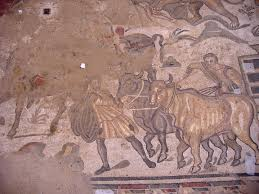
\includegraphics[width=0.65\textwidth]{incomplete.jpg}
 	\end{figure}
\end{frame}

\begin{frame}{Restauration: Was es zu beachten gilt}
\begin{enumerate}
\item{Transparenz ist wichtig. Man muss sagen, welche Teile man zu Beginn hat und durch welche 
Annahmen und Methoden man zu dem Gesamtbild kommt.}\pause
\item{Das Bild das, nach der Restauration entsteht, kann (in Teilen) fehlerhaft sein. Es ist mit Unsicherheit behaftet.}\pause
\item{Je weniger Teile man zu beginn hat bzw. je komplizierter das Bild ist, desto größer ist die Unsicherheit über das Ergebnis.}\pause
\item{Es gibt  viele Möglichkeiten zu dem Ergebnis zu kommen, es gibt nicht den einen richtigen Weg.}\pause
\item{Konstruktiv-kritisches Nachfragen daher ist sinnvoll. Man braucht den Blick von unterschiedlichen Personen (aus verschiedenen Disziplinen)
um die Güte des Bildes beurteilen zu können.}
\end{enumerate}
\end{frame}

\begin{frame}{Gibt es überhaupt ein Muster?}
     \begin{figure}[ht]
 	\centering
 	      
\includegraphics[width=0.6\textwidth]{pattern.jpg}
 	\end{figure}
\end{frame}

\begin{frame}{Können wir aus den gegebenen Informationen etwas schließen?}
     \begin{figure}[ht]
 	\centering
 	      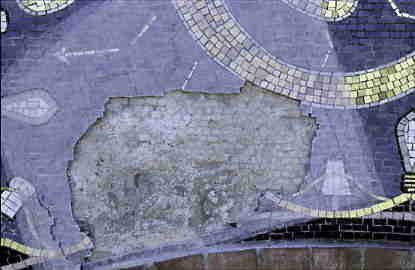
\includegraphics[width=0.65\textwidth]{incomplete2.jpg}
 	\end{figure}
\end{frame}

\begin{frame}{Wie viel darf hier fehlen, damit man eine Chance hat das Muster zu finden?}
     \begin{figure}[ht]
 	\centering
 	      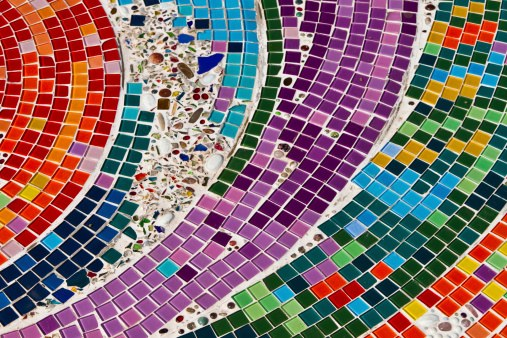
\includegraphics[width=0.65\textwidth]{mosaic-pattern.jpg}
 	\end{figure}
\end{frame}

\begin{frame}{Welche Teile dürfen fehlen, damit man eine Chance hat das Muster zu finden?}
     \begin{figure}[ht]
 	\centering
 	      
\includegraphics[angle=90,width=0.6\textwidth]{patchwork.jpg}
 	\end{figure}
\end{frame}

\begin{frame}{Werkzeugkiste für die Restauration}
Was gehört rein:
\begin{enumerate}
\item{Kreativität und Fingerspitzengefühl }\pause
\item{Sachwissen über den Hintergrund der Daten (der Teile, die man hat)}\pause
\item{Grundlagen der Methoden der empirischen Sozialforschung}\pause
\item{Grundlagen der deskriptiven Statistik, eine gute Beschreibung der Daten ist sehr viel wert}\pause
\item{Grundlagen der Inferenzstatistik, insbesondere der Test- und Schätztheorie}\pause
\item{Die Fähigkeit Statistik-Software zu nutzen}
\end{enumerate}
\end{frame}

\section{Zufallsvorgang}% Fahrmeier-Tutz S. 174, Yudi Pawitan S.4 manchmal ist es auch einfach zu komplex
\begin{frame}{Zufallsvorgang}
\begin{variableblock}{Definition: Zufallsvorgang }{bg=Orchid!30,fg=black}{bg=Plum!30,fg=black}
    	Ein Zufallsvorgang führt zu einem von mehreren, sich gegenseitig ausschließenden Ergebnissen. Es ist vor der Durchführung ungewiss, welches Ergebnis
    	tatsächlich eintreten wird.
\end{variableblock}\pause
\begin{itemize}
\item{Die Ziehung einer Stichprobe ist ein Beispiel für einen Zufallsvorgang. }\pause
\begin{itemize}
\item{ Befragung von Studierenden nach gezahlter monatlicher Miete}\pause
\end{itemize}
\item{Viele Prozesse die wir beobachten können sind Zufallsvorgänge. }
\begin{itemize}
\item{Beispiel: Wie viel Personen nehmen heute an der Vorlesung teil? }\pause
\end{itemize}
\end{itemize}
\end{frame}

\begin{frame}{Zufallsexperiment}
\begin{variableblock}{Definition: Zufallsexperiment}{bg=Orchid!30,fg=black}{bg=Plum!30,fg=black}
    	Bei Beobachtungsstudien, Befragungen oder allgemeinen Stichprobenerhebungen sind im Gegensatz zu Experimenten die
    	Rahmenbedingungen i. a. nicht kontrollierbar bzw. bekannt. Man spricht von einem Zufallsexperiment, wenn ein Zufallsvorgang 
    	unter kontrollierten Bedingungen abläuft und somit unter gleichen Bedingungen wiederholbar ist.
\end{variableblock}
Unter Rahmenbedingungen bzw. Bedingungen sind alle Umstände zu verstehen, die einen Einfluss auf den Vorgang haben.
Das Würfeln ist eine Beispiel für ein Zufallsexperiment.
\end{frame}

\begin{frame}{Chaotisches System}
\begin{variableblock}{Definition: Chaotisches System}{bg=Orchid!30,fg=black}{bg=Plum!30,fg=black}
Oft beschreiben wie unerklärte Phänomen mit Hilfe von probabilistischen Gesetzen,
obwohl man diese Phänomene rein deterministisch beschreiben könnte. Es ist eine Möglichkeit mit Prozessen
umzugehen, die zu komplex sind, um sie einfach vorherzusehen. Es ist dann für uns ungewiss, welches Ereignis
tatsächlich eintreten wird, auch wenn man es theoretisch vorhersagen könnte.
%Often, we impose a probabilistic structure on an unexplained
%phenomenon although the structure of the phenomenon is purely
%deterministic but the underlying mechanism is too complex and
%cannot be recovered from the data, e.g. chaotic systems.
\end{variableblock}
\begin{itemize}
\item{Wir unterscheiden nicht, ob ein Prozess eigentlich deterministisch ist und einfach zu komplex um den Ausgang absehen zu können oder
ob es ein wirklicher stochastischer Prozess ist.}
\item{Pendelbewegungen als auch das Würfeln können als chaotische Systeme verstanden werden.}
\end{itemize}
\end{frame}

\begin{frame}{Zufallsvorgang}
Der Begriff Zufallsvorgang ist daher ein Überbegriff für Zufallsexperimente und chaotische Systeme.
Charakteristisch für den Zufallsvorgang sind zwei Eigenschaften
\begin{enumerate}
\item{Man kennt im Vorfeld bereits die möglichen Ausgänge, wobei unbekannt ist, welcher Eintritt.}
\item{Es hängt ``vom Zufall'' ab, welchen Ausgang man beobachtet.}
\end{enumerate}
\begin{block}{Befragung nach Taschengeld als Zufallsvorgang}
Im Folgenden wollen wir die Normalverteilung nutzen als probabilistisches Gesetzt um die fiktive Befragung
von Kindern in einer Schule nach der Höhe ihres Taschengeldes als Zufallsvorgang zu beschreiben.
\end{block}
\end{frame}

% Durchschnittswert abziehen, dass Verteilung um Null schwankt. Der ist uns bekannt aus der Zeitung

% Zufallsvariable: Beispiel Taschengeld, Beispiel Normalverteilung
\section{Zufallsvorgang am Beispiel}

\begin{frame}{Rückblick: Die Normalverteilung}
Die Normalverteilung ist ein erste Beispiel für ein probabilistisches Gesetzt. (Erklären was eine Verteilung ist)
% Begriff Zufallsvariable Mittag S. 156, FT S. 226
\end{frame}
% Man fragt in einer Schule Schülerinnen und Schüler die Vorbei kommen, danach, wie viel Taschengeld sie bekommen

%\begin{frame}{Was möchte eine statistisches Modell}
%\end{frame}

\begin{frame}{Die unterschiedlichen Formen der Normalverteilung}
        \begin{figure}[ht]
 	\centering
 	      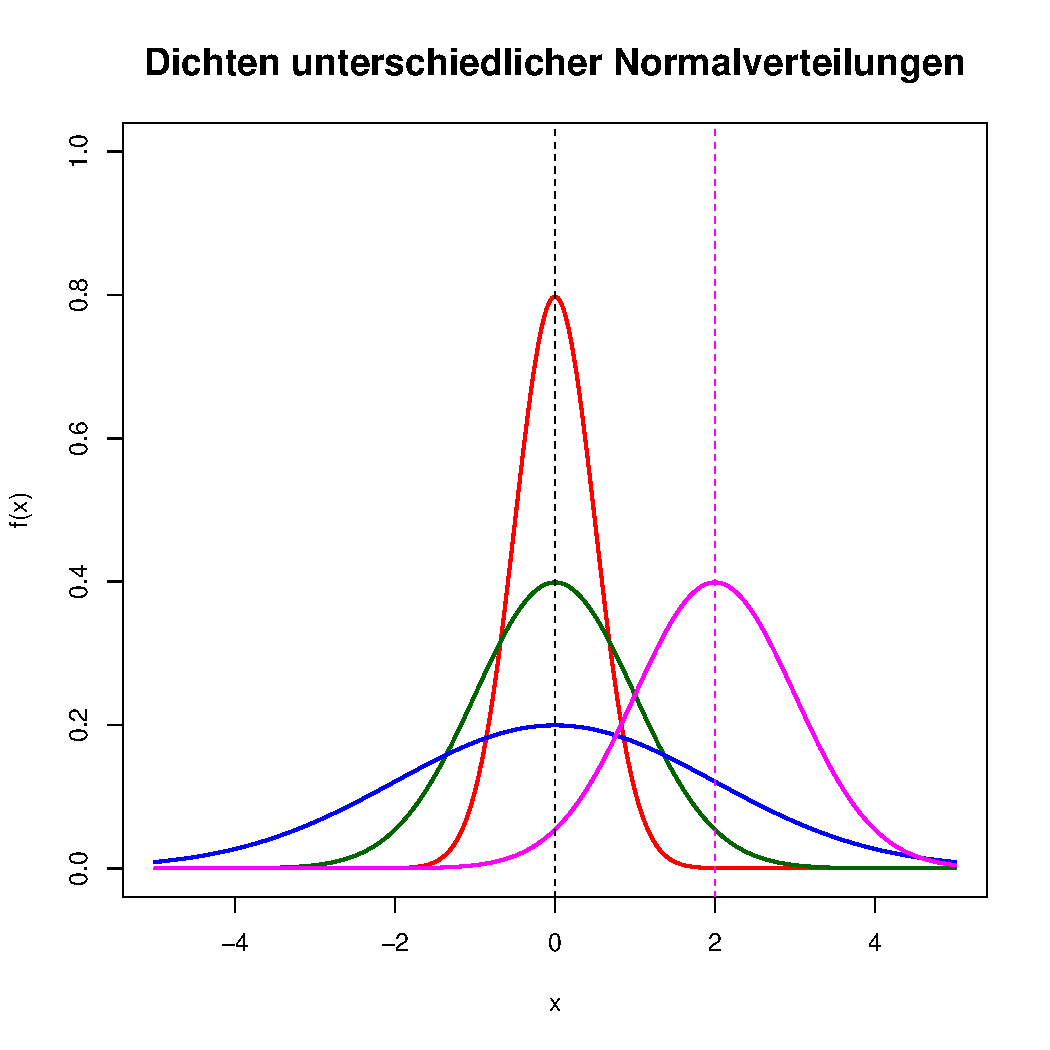
\includegraphics[width=0.65\textwidth]{diffnorm2_leer.pdf}
 	\end{figure}
\end{frame}

\begin{frame}{Was bewirkt eine Veränderung des Mittelwerts?}
        \begin{figure}[ht]
 	\centering
 	      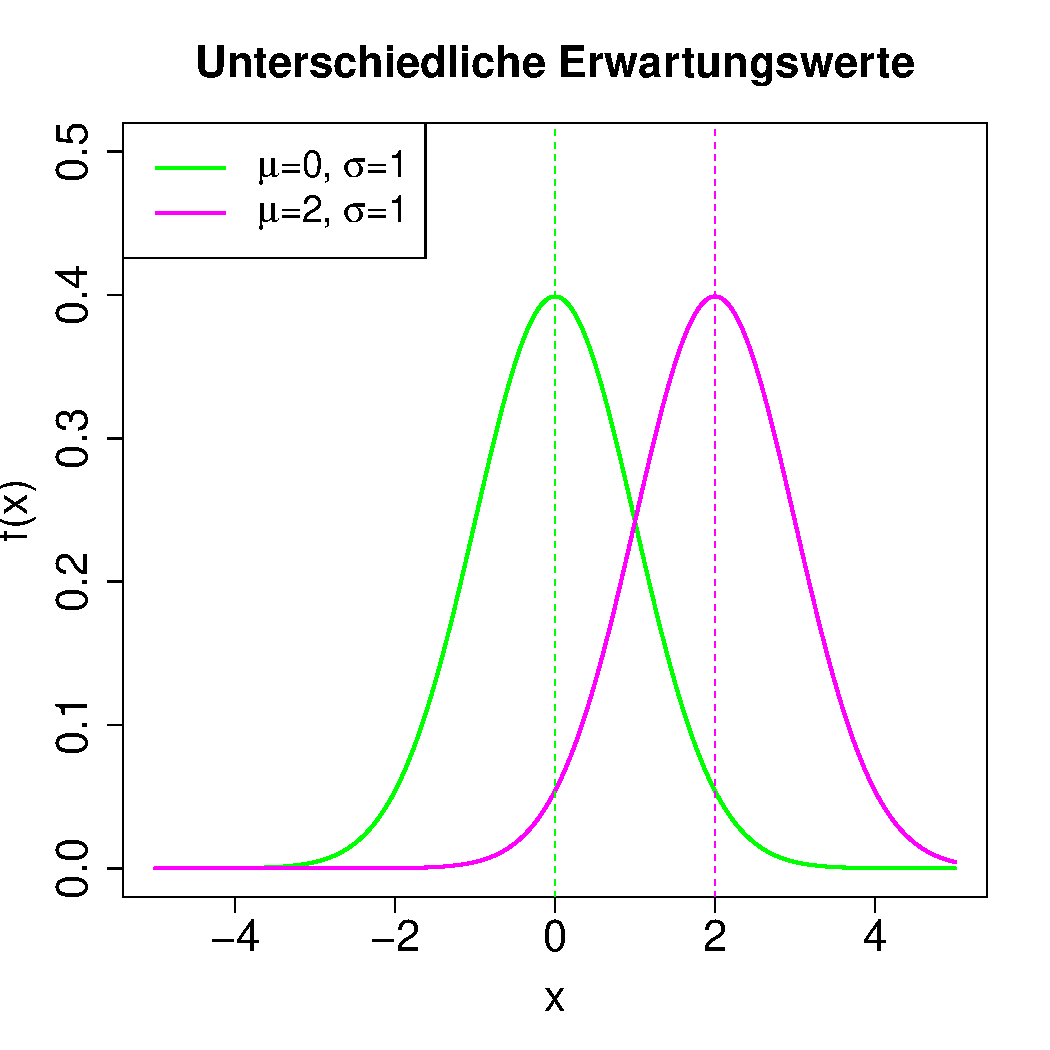
\includegraphics[width=0.65\textwidth]{diffnorm2.pdf}
 	\end{figure}
\end{frame}

\begin{frame}{Was bewirkt eine Veränderung der Standardabweichung?}
        \begin{figure}[ht]
 	\centering
 	      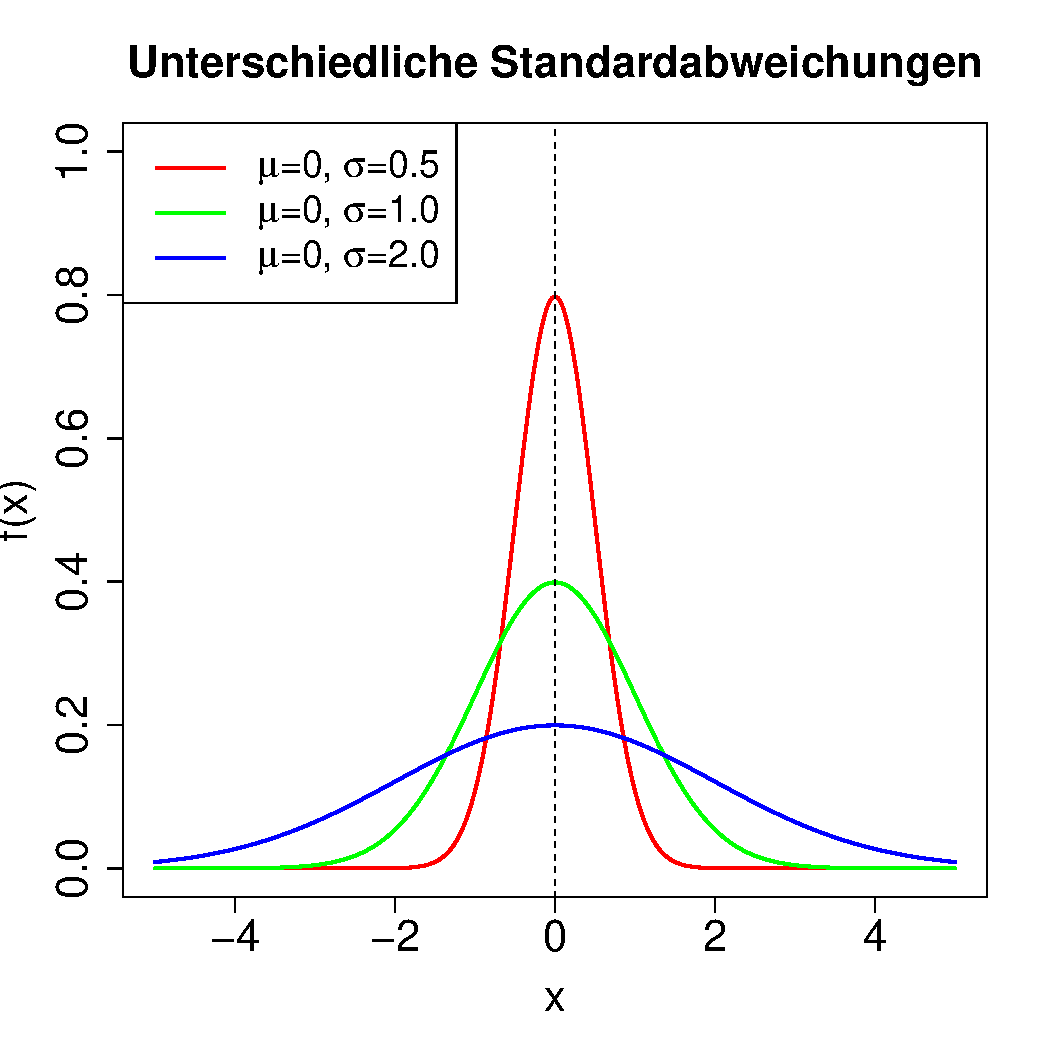
\includegraphics[width=0.65\textwidth]{diffnorm1.pdf}
 	\end{figure}
\end{frame}

% Daten und Modellebene: Unterscheidung finde ich nicht mehr sinnvoll?
% Beispiel: Aufgabe: Ein Punkt auf Bezug zu diesem Wert.
% Umformulieren in: Daten mit Modell in Verbindung bringen: ja oder nein
% Man kann Daten deskriptiv mit Modell in Verbindung bringen

%Wir haben aufgehört mit dem Gruppenunterschied (Jungen-Mädchen: Lesen sie besser)
%Wir fangen wieder an mit Taschengeld (aktueller Bezug: http://www.spiegel.de/lebenundlernen/schule/jungen-bekommen-mehr-taschengeld-als-maedchen-a-1161915.html)
% http://www.spiegel.de/wissenschaft/mensch/taschengeld-gibt-es-wirklich-einen-gender-pay-gap-a-1100475.html
\begin{frame}{Bekommen Jungen mehr Taschengeld als Mädchen?}
Bitte lesen sie die beiden Artikel 
\begin{enumerate}
\item{ \colorbox{yellow!20}{Statistik und Wahrheit - Hauptsache spektakulär} \footnotesize{ \url{http://www.spiegel.de/wissenschaft/mensch/taschengeld-gibt-es-wirklich-einen-gender-pay-gap-a-1100475.html} } 
Erscheinungsdatum: 27.7.2016}
\item{ \colorbox{yellow!20}{ Umfrage: Jungen bekommen mehr Taschengeld als Mädchen} \footnotesize{ \url{http://www.spiegel.de/lebenundlernen/schule/jungen-bekommen-mehr-taschengeld-als-maedchen-a-1161915.html} }
Erscheinungsdatum:  8.8.2017}
\end{enumerate}
\colorbox{green!20}{Machen Sie sich ein paar Stichpunkte zu dem Ergebnis, }
\colorbox{green!20}{dass der zweite Artikel Ihnen Nahe legt und kommentieren Sie es kritisch.}
\end{frame}
\end{document}